\documentclass{article}

\usepackage[utf8]{inputenc}
\usepackage[latin1]{inputenc}
\usepackage[francais]{babel}

\usepackage[left=2cm]{geometry}
\usepackage{amsmath,amssymb,mathrsfs}
\usepackage{graphicx}
\usepackage[table,xcdraw]{xcolor}

\usepackage{enumerate}

\usepackage{tikz}
\usetikzlibrary{shapes,arrows}

\usepackage{fullpage}

\begin{document}

\section*{Examen HPCA}\label{sec:name}
\addcontentsline{toc}{section}{Examen HPCA}

\section*{Exercice 1 - Parrall\'elisation d'un algorithme s\'equentiel}\label{sec:name}
\addcontentsline{toc}{section}{Exercice 1 - Parrall\'elisation d'un algorithme s\'equentiel}

\textbf{1.} \\

\textbf{Syst\`eme de pr\'ec\'edence} :
\begin{table}[h]
\begin{tabular}{lllll}
T1 $\prec$ T2  & T1 $\prec$ T3  &                &               &               \\
T2 $\prec$ T3  & T2 $\prec$ T4  & T2 $\prec$ T5  & T2 $\prec$ T6 & T2 $\prec$ T8 \\
T3 $\prec$ T5  & T3 $\prec$ T7  &                &               &               \\
T4 $\prec$ T6  & T4 $\prec$ T7  & T4 $\prec$ T9  &               &               \\
T5 $\prec$ T10 & T5 $\prec$ T11 & T5 $\prec$ T13 &               &               \\
T6 $\prec$ T8  & T6 $\prec$ T9  & T6 $\prec$ T10 &               &               \\
T7 $\prec$ T11 & T7 $\prec$ T12 &                &               &               \\
T9 $\prec$ T13 &                &                &               &
\end{tabular}
\end{table}

\textbf{Graphe de pr\'ec\'edence} :
\begin{figure}[!h]
    \centering
    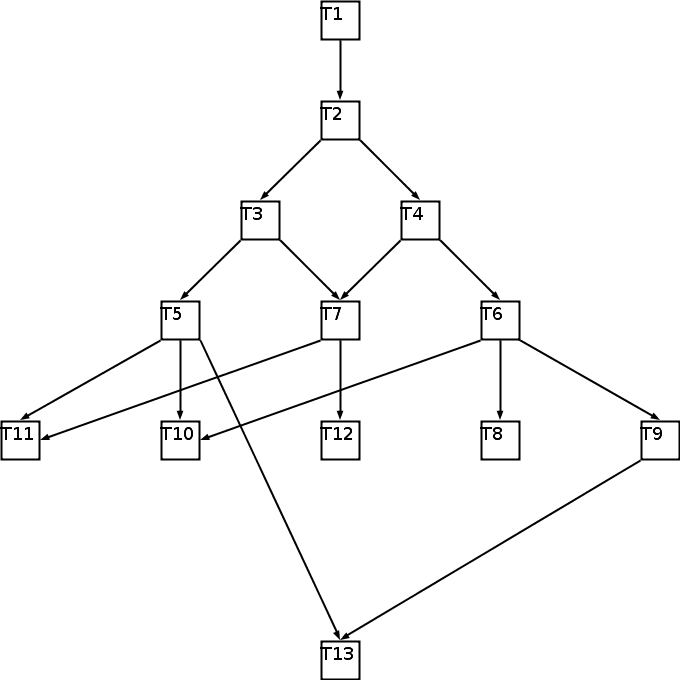
\includegraphics[width=10cm]{graphePrec.png}
\end{figure}

\smallskip
\textbf{2.} \\
\textbf{a. D\'ecomposition par pr\'ec\'ecesseurs}
\begin{center}
\textbf{(1)}\\
\textbf{(2)}\\
\textbf{(3,4)}\\
\textbf{(5,6,7)}\\
\textbf{(8,9,10,11,12)}\\
\textbf{(13)}\\
\end{center}

\textbf{b. D\'ecomposition par successeurs}\\
\begin{center}
  \textbf{(1)}\\
  \textbf{(2)}\\
  \textbf{(4)}\\
  \textbf{(3,6)}\\
  \textbf{(5,7,9)}\\
  \textbf{(8,10,11,12,13)}\\
\end{center}

\textbf{c. Acc\'el\'eration et Efficacit\'e}\\
Les d\'ecompositions par pr\'ec\'ecesseurs et par successeurs ont la m\^eme hauteur (soit 6) donc pour un nombre processeurs optimal nous avons une acc\'el\'eration \'egale \`a :\\
\begin{center}
  $\frac{Tpa}{Tseq} = \frac{6}{13} = 0.46153846153$
\end{center}

Et une efficacit\'e \'egale \`a : \\
\begin{center}
  $\frac{SpeedUp}{NombreProc} = \frac{0.46153846153}{5} = 0.0923076923$\%
\end{center}

\smallskip
\textbf{3.} Le temps d'ex\'ecution de l'algorithme parall\`ele sur une infinit\'e de processeurs est \'egal \`a la hauteur du graphe, soit 6 unit\'e de temps ici.\\

\smallskip
\textbf{4.} Sur une machine \`a 2 processeurs nous pouvons faire la d\'ecompostion suivante :
\begin{center}
  \textbf{(1)}\\
  \textbf{(2)}\\
  \textbf{(3,4)}\\
  \textbf{(5,6)}\\
  \textbf{(7,9)}\\
  \textbf{(8,10)}\\
  \textbf{(11,12)}\\
  \textbf{(13)}\\
\end{center}

Nous avons une hauteur \'egale \`a 8 donc nous avons une borne maximale \'egale \`a 8 unit\'e de temps.\\

\smallskip
\textbf{5.} Nous ne pouvons pas trouver de d\'ecomposition sur 2 processeurs demandant un temps inf\'erieur \`a cette borne car les deux premi\`eres t\^aches ne sont pas parall\'elisable.\\

\section*{Exercice 2 - Diffusion sur une grille}\label{sec:name}
\addcontentsline{toc}{section}{Exercice 2 - Diffusion sur une grille}


\end{document}
